
\subsection{Arithmetic Circuits}
Sequences of operations over field elements and variables can be neatly represented by
\emph{arithmetic circuits}.
\begin{definition}[Arithmetic circuit]
	Given a field \(\mathbb{F}\), some \(n, m \in \mathbb{N}\), some constants
	\(a_{1, 1}, \dots, a_{m, n} \in \mathbb{F}\), and some variables \(x_1, \dots, x_n \) over
	\(\mathbb{F}\), an \emph{implicit arithmetic circuit} over \(\mathbb{F}\) is any formula:
	\begin{align*}
		 & \phi \equiv c                     &  & \textnormal{with \(c \in \mathbb{F}\)}
		\\
		 & \phi \equiv x                     &  & \textnormal{with \(x\) variable over
			\(\mathbb{F}\)}
		\\
		 & \phi \equiv \phi_1^c              &  & \textnormal{with \(c \in \mathbb{F}\) and
			\(\phi_1 \neq \phi \) arithmetic circuit}
		\\
		 & \phi \equiv \phi_1 \oplus \phi_2  &  & \textnormal{with \(\phi_1 \neq \phi, \phi_2 \neq
			\phi \)
			arithmetic circuits}
		\\
		 & \phi \equiv \phi_1 \otimes \phi_2 &  & \textnormal{with \(\phi_1 \neq \phi, \phi_2 \neq
			\phi \)
			arithmetic circuits}
		\\
		 & \phi \equiv \phi_1, \phi_2        &  & \textnormal{with \(\phi_1 \neq \phi, \phi_2 \neq
			\phi \)
			arithmetic circuits}
	\end{align*}
	An arithmetic circuit which does not contain multiplications and exponentiations by constants
	is called \emph{(explicit) arithmetic circuit}.
\end{definition}

\noindent Every arithmetic circuit can be represented by a Directed Acyclic Graph (DAG),
where the vertices are labeled either with a variable name (\emph{variable vertices}), a constant
from the field (\emph{constant vertices}) or one of the operations \(\oplus \)
(\emph{addition vertices}, denoted \(\phi_\oplus \)) and \(\otimes \) 
(\emph{multiplication vertices}, denoted \(\phi_\otimes \)).
With an analogy to digital circuits, vertices are also called \emph{gates}.
Only addition and multiplication vertices have incoming edges (exactly two), which represent the
inputs of the operation, while the outgoing edge will represent the result.
Vertices without ingoing edges are called \emph{input vertices}, while vertices without outgoing
edges are called \emph{output vertices}, together they are denoted \(\phi_{IO}\).

It is possible, without affecting the expressive power, to transform an implicit arithmetic circuit
into an explicit one by replacing exponentiations (multiplications) by some constant \(c\) with a
a sequence of \(c\) multiplications (additions)\footnote{However, this transformation can affect
	the succintness of a circuit and its DAG (unrolling \(x^c\) or \(cx\) requires \(\Theta(2^c)\)
	space), but this won't be a problem for us.}.
\begin{figure}
	\centering
	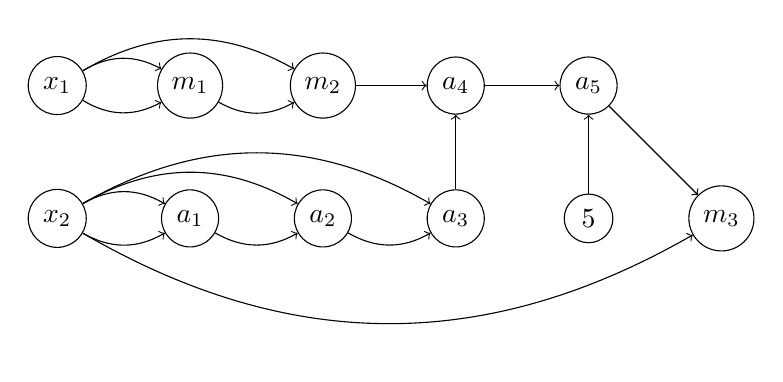
\begin{tikzpicture}[node distance={48pt}, node/.style = {draw, circle}]
		\node[node] (x1) {\(x_1\)};
		\node[node] (x2) [below of=x1] {\(x_2\)};
		\node[node] (m1) [right of=x1] {\(m_1\)};
		\node[node] (m2) [right of=m1] {\(m_2\)};
		\node[node] (a1) [right of=x2] {\(a_1\)};
		\node[node] (a2) [right of=a1] {\(a_2\)};
		\node[node] (a3) [right of=a2] {\(a_3\)};
		\node[node] (a4) [right of=m2] {\(a_4\)};
		\node[node] (a5) [right of=a4] {\(a_5\)};
		\node[node] (5) [below of=a5] {\(5\)};
		\node[node] (m3) [right of=5] {\(m_3\)};
		\draw[->] (x1) to [bend left] (m1);
		\draw[->] (x1) to [bend right] (m1);
		\draw[->] (x1) to [bend left] (m2);
		\draw[->] (m1) to [bend right] (m2);
		\draw[->] (x2) to [bend left] (a1);
		\draw[->] (x2) to [bend left] (a2);
		\draw[->] (x2) to [bend left] (a3);
		\draw[->] (x2) to [bend right] (a1);
		\draw[->] (a1) to [bend right] (a2);
		\draw[->] (a2) to [bend right] (a3);
		\draw[->] (m2) to (a4);
		\draw[->] (a3) to (a4);
		\draw[->] (a4) to (a5);
		\draw[->] (5) to (a5);
		\draw[->] (a5) to (m3);
		\draw[->] (x2) to [bend right] (m3);

	\end{tikzpicture}
	\caption{DAG of the circuit in Example~1.
		We have the two variable/input vertices \(x_1\) and \(x_2\), the constant vertex \(5\), the
		addition vertices \(a_1, \dots, a_5\) and the multiplication vertices \(m_1, m_2\) and
		\(m_3\),
		which is also an output vertex.}\label{fig:example_dag}
\end{figure}
\begin{example}\label{ex:circuit}
	Let's consider the following implicit arithmetic circuit over \(\mathbb{F}_{13}\):
	\[\phi = x_{2}\left(x_{1}^{3} + 4x_{2} + 5\right)\]
	We can unroll it into an equivalent (explicit) arithmetic circuit:
	\[\widehat{\phi} = x_{2}\left(x_{1}x_{1}x_{1} + x_{2} + x_{2} + x_{2} + x_{2} + 5\right)\]
	And draw the associated DAG, which is shown in Figure~\ref{fig:example_dag}.
\end{example}
